\section{Aim 1}

\subsection{Rationale}

Aim 1 is centered around the creation and modeling of the TCP material. There are multiple methods used to make this process consistent and reliable. Most notably those described in \cite{wu_compact_2017}, where the TCP actuation method is used to manipulate a humanoid hand. With the purpose of simplfication of the creation/modeling process, a precursor fiber with similar specifications to that of the aforementioned article will be purchased.

In order to achieve a consistent fabrication process, the TCP will be spun using an automated system; similar to that of a rope making machine. The system will be configurable to a set number of rotations, and a set RPM speed, as well as having connections for an adjustable counter-weight which will be used as the third and final configuration input when making the material. Once the fabrication process is created and checked for consistency, data will be collected on the actuation capabilities of the string with varying configuration inputs. A setup will be chosen based on the data collected.

The next step is to derive a control model formula which can represent the tension exhibited by a single strand of the TCP with inputs of current $[Amps]$ and time $[seconds]$. The constant parameters of the system will ideally be the same as the parameters used when creating the TCP string, but will require more testing to legitimize. Because TCP is actuated via heat generation, the system dynamics will be time-dependent, and will be discussed in the next section.

Finally, a controller will be implemented (figure \ref{fig:control_diagram}), ideally using the aforementioned model formula. The current plan is to utilize an optimal control policy with the inclusion of an accurate model. In cases where the model cannot be applied, a simpler sub-optimal policy may be used instead. Both options are feasible.

\begin{figure}[ht]
	\centering
	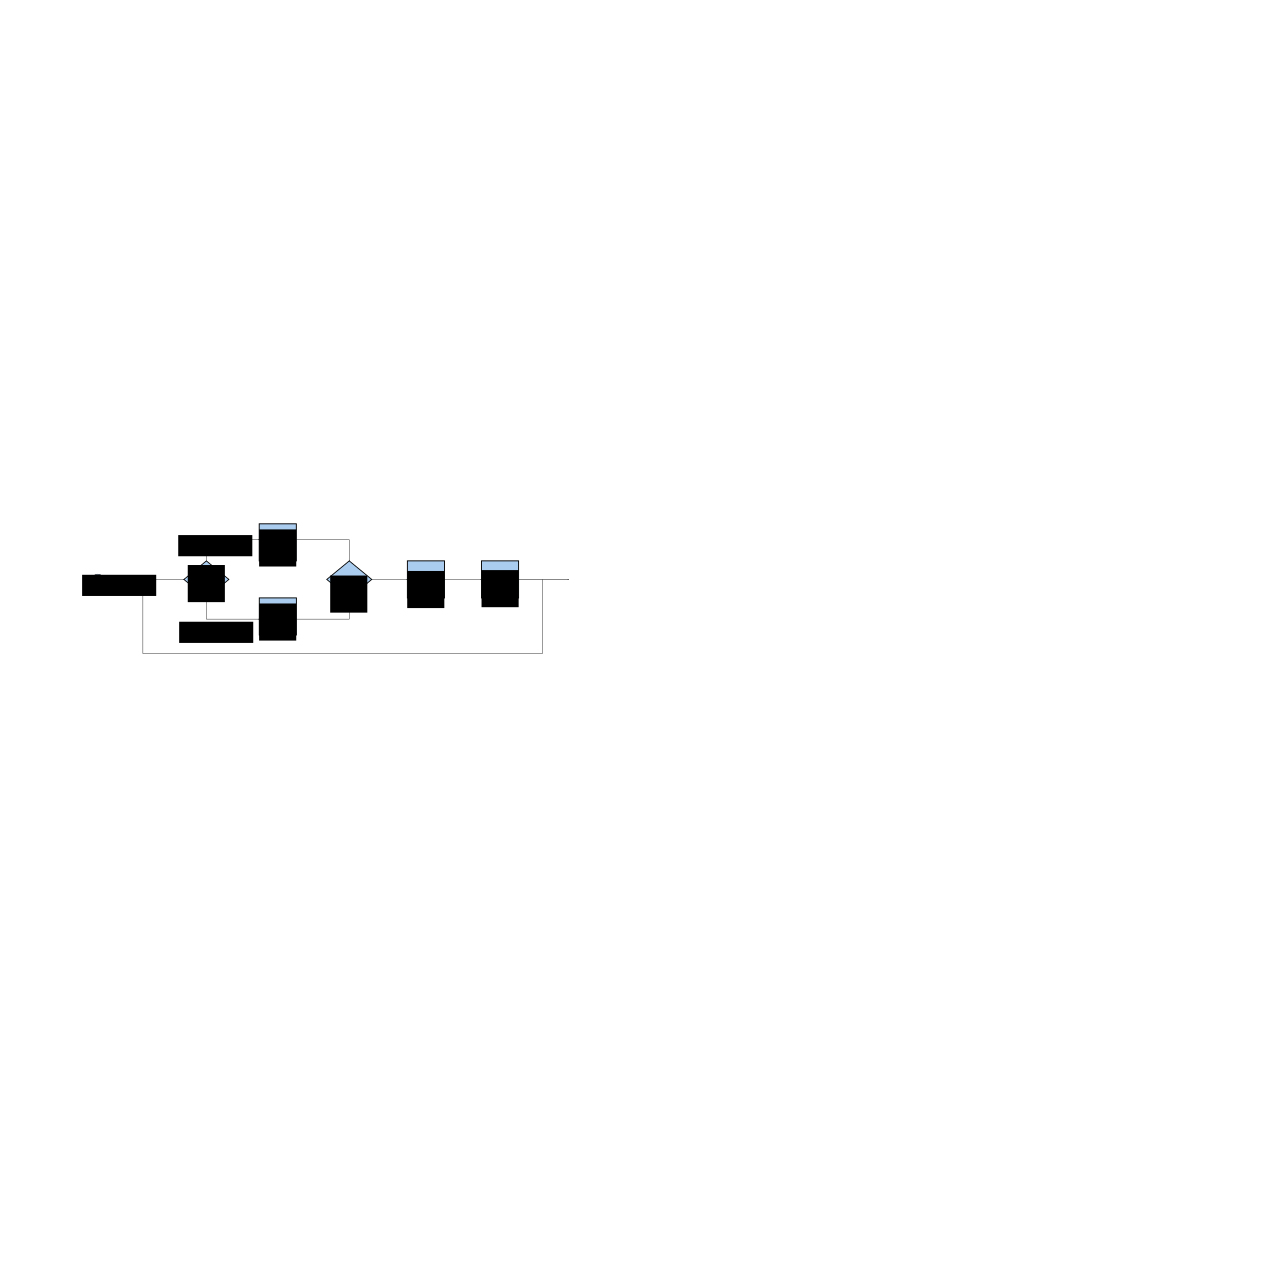
\includegraphics[scale=0.30]{control_diagram}
	\caption{AEI System Control Diagram}
	\label{fig:control_diagram}
\end{figure}

Figure \ref{fig:control_diagram} shows the planned controller structure. The user-input block is a set of parameters received from the user during runtime. This will tell the device whether the user is in manual or automated operation modes, and will split into two similarly structured decision branches. With a desired trjectory chosen, the tracking controller will decide the necessary current value before uploading the results to the system dynamics and continuing.

\subsection{Approach}

	\subsubsection{Hypothesis/Timeline}

The fabrication of the TCP material will be facilitated through an in-house rope making machine which are standard and can be automated relatively easily. The wire of choice will be silver-coated nylon 66 wire, similar to that used in the initial prototype. The control board of choice for the automation will be an Arduino Uno, and will be used to control the RPM of the machine, as well as the number of spins. The counter-weight attached to the machine can also be adjusted for further variations. For consistency, the length of the TCP created at a given time will be held constant, and will be heat-treated and trained using the research verified by [CITE SOURCE FOR FABRICATION].

Modeling of the TCP system will be the most difficult of the steps discussed in this research. Here, the formula for the TCP dynamics will be simplified to take the inputs current and voltage, and output the tension created after a certain period of time. This is achieved in the research conducted here [CITE MODELING ARTICLE]. The model will be compared to the real TCP using a tension measurement device, and by holding the current and voltage constant over the intended period of time. In this way, the error between the model and the real system can be evaluated at varying configuration settings. With tension calculated, the system then be directly compared to a solely tension-driven actuation system. This effectively turns the model from a current (input) to tension (output) calculation, to a current (input) to motion (output) formula.

The controller for the system will ideally be model-dependent. It is understood that model-dependent controllers, when accurately tuned, create the most effective system controllers and are more reliable and robust then model-independent alternatives. Also, considering the time-dependence of the TCP system, the use of MPC will be prioritized because of its ability to look into future states and solve for the optimal set of inputs at a given point in time.

	\subsubsection{Modeling Techniques}
	\section{Modeling Techniques}
\label{sect:modeling_techniques}
	
	As derived in \textit{Modeling of twisted and coiled polymers (TCP) muscle based on phenomenological approach} by Farzad Karami and Yonas Tadesse. For modeling of TCP actuators, the following steps are used to approximate the temperature and displacement of the material based on a given current, TCP dimensions and load.

	The change in resistance with respect to temperature is shown in Equation \ref{eq:tcp_resistance} below.
	
	\begin{equation}
	\label{eq:tcp_resistance}
		R(T) = R_{0} (1 + \alpha (T - T_{0}))
	\end{equation}
	
	Where $R(T)$ represents the current resistance in $[ohms]$, $R_{0}$ is the resistance at a reference temperature, $T$ is the current temperature of the TCP, and $T_{0}$ is the reference temperature. Finally, $\alpha$ is the coefficient of thermal expansion (CTE). For the purpose of manipulating tension using the TCP, a material with a negative CTE was chosen. It is further explored that the elastic modulus (E) is also determined by temperature.
	
	For equation \ref{eq:tcp_resistance} to be used accurately during modeling the change in temperature must also be approximated. This is completed below.
	
	\begin{equation}
	\label{eq:tcp_temperature}
		T - T_{\infty} =
			- \frac{R_{0} i^{2}}{-h A + R_{0} i_{2} \alpha}
			\left(
				1 -
				\exp^{\frac{-h A + R_{0} i_{2} \alpha}{m c_{p}}} t
			\right)
	\end{equation}
	
	Where $T_{\infty}$ is the ambient temperature, $i$ is the operating current, $h$ is the coefficient of heat convection, $A$ is the exposed TCP surface area, $m$ is the TCP mass, $c_{p}$ is the specific heat capacity, and $t$ is the time-passed. This is used to approximate the temperature, $T$, of the TCP with respect to a given current, $i$, and time, $t$.
	
	Using Equation \ref{eq:tcp_temperature} in combination with the function for $E$ (equation \ref{eq:tcp_elastic_modulus} and along with the dimensions of the TCP material, the displacement of the TCP can be calculated using the set of equations shown below.
	
	\begin{equation}
	\label{eq:tcp_elastic_modulus}
		E(T) = a_{1} T^{a_{2}} + a_{3}
	\end{equation}
	
	\begin{equation}
	\label{eq:tcp_displacement_elastic}
		\Delta_{el} = \frac{F}{k}
	\end{equation}
	
	\begin{equation}
	\label{eq:tcp_displacement_thermal}
		\Delta_{th} = \delta H
		\begin{matrix}			
			= \frac{L \delta L - \pi D \delta D}{\sqrt{L^{2} - \pi D^{2}}} \\
			= \frac{L^{2}_{0}}{H_{0}} \alpha_{L} (T - T_{0}) - \frac{pi D^{2}_{0}}{H_{0}} \alpha_{T} (T - T_{0})
		\end{matrix}
	\end{equation}
	
	\begin{equation}
	\label{eq:tcp_displacement}
		\Delta H = H_{0} - \Delta_{th} + \Delta_{el}
	\end{equation}
	
	Equation \ref{eq:tcp_elastic_modulus} represents a fitted function for the elastic modulus of a single string of TCP at a given temperature. Equation \ref{eq:tcp_displacement_elastic} is the displacement of the TCP with respect to the load and equation \ref{eq:tcp_displacement_thermal} is the displacement based on the CTE. Finally, equation \ref{eq:tcp_displacement} is the total displacement based on the previous two equations.
	
	Here, $a_{1}$, $a_{2}$ and $a_{3}$ are the fitted curve coefficients, $F$ is the load on the TCP, $k$ is the elastic coefficient (not derived here), $L_{0}$ is the initial TCP stretched length, $H_{0}$ is the initial TCP coiled length, $D_{0}$ is the diameter of the coiled wire, $\alpha_{L}$ is the longitudinal CTE, and $\alpha_{T}$ is the transverse CTE. The suse of these equations allow for the approximation of the TCP length at a given point in time.
	
	The issue that arises here is the assumption that the load, $F$, is constant. For the purpose of implementation in AEI, the tension must be dynamic in the modeling. This issue will be addressed during the modeling 
	
	\subsubsection{Experimental Process}

\subsection{Risks and Alternatives}

It is understood that all of the steps taken in this portion of the development process are subject to considerable obstacles. That said, each of the discussed approaches have alternative methods of attack which should still achieve the overarching goals of the project.

In the case of the fabrication. It is likely that the TCP string may be too thin, inconsistent string could be purchased, or the machine itself may be too intricate to make/program in-house. In the scenario of thin or inconsistent string, there are many companies that make the intended wire and ordering thicker/more consistent silver-coated polymer wire is possible. Once a certain brand of wire proves sufficient, it will be ordered in bulk and used for the remainder of the project. If the machine proves too intricate to make by hand, it is also possible to order small scale rope making machines online.

Since TCP is a relatively new form of actuation and is time-dependent, verified methods of modeling are not easily found. Here, the equations derived from the research of Farzad Karami and Yonas Tadesse in [CITE MODELING ARTICLE] will be used to supplement the formulations found in-house. In the extreme case that the model cannot be derived analytically, it is also possible to train a neural network to produce the intended behavior. This would involve considerably more data on configuration details, but is very possible and has been done for likewise projects in the past [SE3-nets ARTICLE, YANG AND MENG ARTICLE].